\documentclass[10pt,aspectratio=169]{beamer}
\usetheme{Boadilla}
\usecolortheme{dove}

\usepackage{amsmath}
\usepackage{booktabs}
\usepackage{array}
\usepackage{tikz}
\usetikzlibrary{arrows.meta,positioning}

\providecommand{\AnalyticalClaimCount}{13}
\providecommand{\AnalyticalIdentityCount}{9}
\providecommand{\BootstrapReplications}{1000}
\providecommand{\BootstrapBlockLength}{4}
\providecommand{\SimultaneousBandLevel}{95}
\providecommand{\LineThetaObject}{12}
\providecommand{\LineObservedOutput}{19}
\providecommand{\LineTechniqueChoice}{63}
\providecommand{\LineAccumulatedPath}{75}
\providecommand{\LinePreferredRecovery}{224}
\providecommand{\LineProfitForm}{567}
\providecommand{\LineHarrodianBenchmark}{411}
\providecommand{\HashSthirtyThree}{8c903fef31}
\providecommand{\HashIdentificationRule}{b5b73e3e03}
\providecommand{\HashChapterOutline}{0c82845424}


\setbeamertemplate{navigation symbols}{}
\setbeamertemplate{headline}{}
\setbeamercolor{titlelike}{parent=structure,bg=gray!10}
\setbeamercolor{item}{fg=gray!80}
\setbeamercolor{block title}{bg=gray!20,fg=black}
\setbeamercolor{block body}{bg=gray!5,fg=black}
\setbeamercolor{alertblock title}{bg=red!16,fg=black}
\setbeamercolor{alertblock body}{bg=red!4,fg=black}
\setlength{\parskip}{0pt}
\setbeamertemplate{itemize/enumerate body begin}{\vspace{-0.15em}}
\setbeamertemplate{itemize/enumerate subbody begin}{\vspace{-0.15em}}

\definecolor{pathred}{HTML}{B2182B}
\definecolor{pathblue}{HTML}{2166AC}
\definecolor{pathgreen}{HTML}{4D9221}
\definecolor{pathpurple}{HTML}{762A83}

\newcolumntype{L}[1]{>{\raggedright\arraybackslash}p{#1}}
\newcommand{\LR}{\mathrm{LR}}
\newcommand{\sourcefooter}[1]{%
  \par\vfill{\tiny\color{gray!70}Analytical source: #1}\vspace{-0.35em}}

\title[Identifying long-run $\theta_t$]{Identifying the Long-Run Transformation Elasticity}
\subtitle{Path-dependent technique choice and accumulation regimes}
\author{Dissertation Chapter 2}
\date{July 2026}

\setbeamertemplate{footline}{%
  \leavevmode%
  \hbox{%
  \begin{beamercolorbox}[wd=.82\paperwidth,ht=2.4ex,dp=1.1ex,leftskip=1em]{author in head/foot}%
    \insertshorttitle\hfill Analytical identification addendum
  \end{beamercolorbox}%
  \begin{beamercolorbox}[wd=.18\paperwidth,ht=2.4ex,dp=1.1ex,center]{date in head/foot}%
    \insertframenumber/\inserttotalframenumber
  \end{beamercolorbox}}%
}

\begin{document}

% Main 1
\begin{frame}{The object is a long-run derivative, not an annual ratio}
  \begin{columns}[T,onlytextwidth]
    \begin{column}{0.63\textwidth}
      \begin{block}{Structural object}
        \centering
        \Large
        $\displaystyle
        \theta_t^{\LR}
        =
        \left.
        \frac{\partial\ln Y_t^p}{\partial\ln K_t^{cap}}
        \right|_{\mathcal M^{\LR}}$
      \end{block}
      \begin{block}{Counterfactual encoded by the derivative}
        Increase productive capital marginally while holding the long-run distributive state and the technique inherited by the new installation fixed.
      \end{block}
    \end{column}
    \begin{column}{0.34\textwidth}
      \begin{alertblock}{Different object}
        \centering
        \Large $\displaystyle \vartheta_t^{path}=\frac{g_t^p}{g_t^{cap}}$

        \vspace{0.6em}\normalsize
        This ratio evaluates one observed annual direction of accumulation. It does not identify the structural derivative.
      \end{alertblock}
    \end{column}
  \end{columns}
  \begin{block}{Identification target}
    What must be estimated is the coefficient vector that governs the marginal capacity payoff of new accumulation along the long-run manifold.
  \end{block}
  \sourcefooter{Theta-recovery specification ledger, source line \LineThetaObject}
\end{frame}

% Main 2
\begin{frame}{Observed output mixes capacity formation with realized use}
  \begin{block}{Accounting separation}
    \centering
    \Large $y_t=y_t^p+\log\mu_t$
  \end{block}

  \vspace{0.5em}
  \centering
  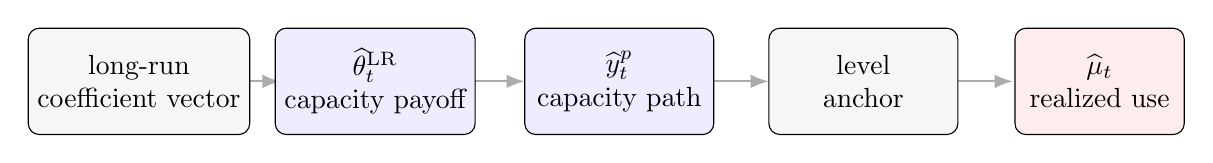
\begin{tikzpicture}[>=Latex, every node/.style={align=center}]
    \draw[->,thick,gray!65] (2.15,0) -- (2.85,0);
    \draw[->,thick,gray!65] (5.25,0) -- (5.95,0);
    \draw[->,thick,gray!65] (8.35,0) -- (9.05,0);
    \draw[->,thick,gray!65] (11.45,0) -- (12.15,0);
    \node[draw,rounded corners,fill=gray!7,minimum width=2.15cm,minimum height=1.35cm] at (1.05,0)
      {long-run\\coefficient vector};
    \node[draw,rounded corners,fill=blue!7,minimum width=2.40cm,minimum height=1.35cm] at (4.05,0)
      {$\widehat\theta_t^{\LR}$\\capacity payoff};
    \node[draw,rounded corners,fill=blue!7,minimum width=2.40cm,minimum height=1.35cm] at (7.15,0)
      {$\widehat y_t^p$\\capacity path};
    \node[draw,rounded corners,fill=gray!7,minimum width=2.40cm,minimum height=1.35cm] at (10.25,0)
      {level\\anchor};
    \node[draw,rounded corners,fill=red!7,minimum width=2.15cm,minimum height=1.35cm] at (13.25,0)
      {$\widehat\mu_t$\\realized use};
  \end{tikzpicture}

  \vspace{0.8em}
  \begin{alertblock}{The residual is not the denominator}
    Residual stationarity admits a long-run relation. Only the reconstructed and anchored $y_t^p$ supplies the denominator from which $\mu_t$ is calculated.
  \end{alertblock}
  \sourcefooter{Distribution-conditioned identification rule, source lines \LineObservedOutput\ and following}
\end{frame}

% Main 3
\begin{frame}{Persistent distribution selects technique before installation}
  \begin{columns}[T,onlytextwidth]
    \begin{column}{0.57\textwidth}
      \begin{block}{Long-run technique choice}
        \centering
        $\displaystyle
        q_t^*=\arg\max_q\bigl[a(q)-q\pi_t^{\LR}\bigr]$

        \vspace{0.55em}
        \Large $a'(q_t^*)=\pi_t^{\LR}=1-\omega_t^{\LR}$
      \end{block}
      \begin{itemize}\small
        \item $q_t^*$ is selected using the distributive state expected to persist over the life of the installation.
        \item The selection occurs before the corresponding capital enters the productive stock.
      \end{itemize}
    \end{column}
    \begin{column}{0.40\textwidth}
      \begin{block}{Separate the horizons}
        \centering
        $\displaystyle \omega_t=\omega_t^{\LR}+\omega_t^{SR}$
        \vspace{0.3em}

        \begin{tabular}{@{}L{0.34\linewidth}L{0.58\linewidth}@{}}
          $\omega_t^{\LR}$ & selects technique for new accumulation \\
          \addlinespace[0.5em]
          $\omega_t^{SR}$ & affects realized output and utilization without repricing the installed stock
        \end{tabular}
      \end{block}
    \end{column}
  \end{columns}
  \begin{alertblock}{Economic implication}
    Contemporaneous wage-share noise cannot be allowed to make the productive capacity of yesterday's capital jump today.
  \end{alertblock}
  \sourcefooter{Theta-recovery ledger, technique-choice condition at source line \LineTechniqueChoice}
\end{frame}

% Main 4
\begin{frame}{New investment inherits yesterday's selected technique}
  \centering
  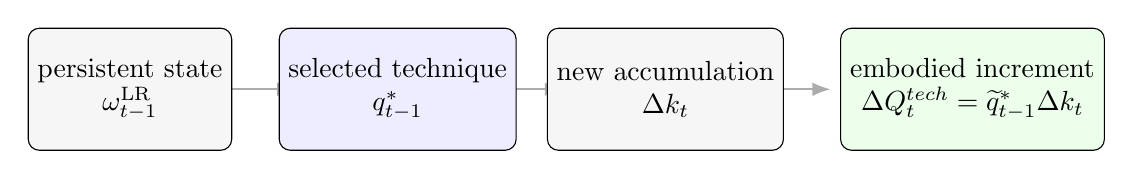
\begin{tikzpicture}[>=Latex, every node/.style={align=center}]
    \draw[->,thick,gray!65] (2.55,0) -- (3.35,0);
    \draw[->,thick,gray!65] (5.95,0) -- (6.75,0);
    \draw[->,thick,gray!65] (9.35,0) -- (10.15,0);
    \node[draw,rounded corners,fill=gray!7,minimum width=2.55cm,minimum height=1.55cm] at (1.25,0)
      {persistent state\\$\omega_{t-1}^{\LR}$};
    \node[draw,rounded corners,fill=blue!7,minimum width=2.55cm,minimum height=1.55cm] at (4.65,0)
      {selected technique\\$q_{t-1}^*$};
    \node[draw,rounded corners,fill=gray!7,minimum width=2.55cm,minimum height=1.55cm] at (8.05,0)
      {new accumulation\\$\Delta k_t$};
    \node[draw,rounded corners,fill=green!8,minimum width=3.35cm,minimum height=1.55cm] at (11.95,0)
      {embodied increment\\$\Delta Q_t^{tech}=\widetilde q_{t-1}^*\Delta k_t$};
  \end{tikzpicture}

  \vspace{1em}
  \begin{columns}[T,onlytextwidth]
    \begin{column}{0.48\textwidth}
      \begin{block}{Installed stock}
        Capital already in place retains the technique selected when it was installed. A change in $\omega_t^{\LR}$ does not revalue its physical capacity.
      \end{block}
    \end{column}
    \begin{column}{0.48\textwidth}
      \begin{block}{New layer of the stock}
        Only $\Delta k_t$ receives the technique weight inherited from $t-1$. The capacity path therefore records the sequence of past installation choices.
      \end{block}
    \end{column}
  \end{columns}
  \sourcefooter{Theta-recovery ledger, causal ordering and accumulated-path construction}
\end{frame}

% Main 5
\begin{frame}{Accumulation turns technique choice into a long-run state}
  \begin{block}{Technique-centered accumulated path}
    \centering
    $\displaystyle
    \widetilde q_t^*=q_t^*-\bar q^{*,\LR},
    \qquad
    Q_t^{tech}=\sum_{s\le t}\widetilde q_{s-1}^*\Delta k_s$
  \end{block}
  \begin{columns}[T,onlytextwidth]
    \begin{column}{0.49\textwidth}
      \begin{block}{What the state remembers}
        \small
        \begin{tabular}{@{}L{0.32\linewidth}L{0.60\linewidth}@{}}
          high $q_{s-1}^*$ & accumulation installed with a technique above the long-run reference \\
          \addlinespace[0.6em]
          low $q_{s-1}^*$ & accumulation installed with a technique below the reference \\
          \addlinespace[0.6em]
          no $\Delta k_s$ & no new technique is embodied in that period
        \end{tabular}
      \end{block}
    \end{column}
    \begin{column}{0.48\textwidth}
      \begin{block}{Centering changes the basis, not capacity}
        \small
        $\displaystyle
        Q_t^{raw}
        =Q_t^{tech}+\bar q^{*,\LR}(k_t-k_0)$

        \vspace{0.5em}
        $\displaystyle
        \beta_K^{centered}
        =\beta_K^{raw}+\beta_Q\bar q^{*,\LR}$
      \end{block}
      \begin{alertblock}{Interpretation}
        $\beta_K^{centered}$ is the capacity elasticity at the reference technique.
      \end{alertblock}
    \end{column}
  \end{columns}
  \sourcefooter{Theta-recovery ledger, accumulated path at source line \LineAccumulatedPath}
\end{frame}

% Main 6
\begin{frame}{The cointegrating vector recovers $\theta_t$ at every date}
  \centering
  \large $y_t=\alpha+\beta_K k_t+\beta_Q Q_t^{tech}+\varepsilon_t$
  \vspace{0.35em}
  \begin{columns}[T,onlytextwidth]
    \begin{column}{0.65\textwidth}
      \begin{block}{Differentiate the reconstructed capacity path}
        \centering
        \begin{align*}
          \Delta y_t^p
          &=\beta_K\Delta k_t+\beta_Q\Delta Q_t^{tech} \\
          &=\left(\beta_K+\beta_Q\widetilde q_{t-1}^*\right)\Delta k_t, \\
          \therefore\quad
          \theta_t^{\LR}
          &=\beta_K+\beta_Q\widetilde q_{t-1}^*.
        \end{align*}
      \end{block}
    \end{column}
    \begin{column}{0.32\textwidth}
      \small\textbf{Estimated once}\par
        $\alpha$, $\beta_K$, and $\beta_Q$ belong to the long-run coefficient vector.

      \vspace{0.8em}
      \textbf{Reconstructed each date}\par
        The lagged technique state maps the fixed vector into the historical $\theta_t^{\LR}$ path.
    \end{column}
  \end{columns}
  \vspace{0.35em}
  \raggedright\textbf{Identification verdict:} Persistence enters through the accumulated installation state, not through a sequence of unrelated annual coefficients.
  \sourcefooter{Theta-recovery ledger, preferred recovery equation at source line \LinePreferredRecovery}
\end{frame}

% Main 7
\begin{frame}{The profit-share formula is the reduced form of embodied technique choice}
  \begin{block}{Affine long-run technique selection}
    \centering
    \Large $q_{t-1}^*=a+b\pi_{t-1}^{\LR}$
  \end{block}
  \begin{block}{Substitution into the accumulated-path derivative}
    \centering
    \begin{align*}
      \theta_t^{\LR}
      &=\beta_K+\beta_Q\left(q_{t-1}^*-\bar q^{*,\LR}\right)\\
      &=\underbrace{\left[\beta_K+\beta_Q(a-\bar q^{*,\LR})\right]}_{\theta_1}
        +\underbrace{\beta_Qb}_{\theta_2}\pi_{t-1}^{\LR}\\
      &\equiv\theta_1+\theta_2\pi_{t-1}^{\LR}.
    \end{align*}
  \end{block}
  \begin{columns}[T,onlytextwidth]
    \begin{column}{0.48\textwidth}
      \textbf{$\theta_1$:} capacity payoff at the reference long-run distributive state.
    \end{column}
    \begin{column}{0.48\textwidth}
      \textbf{$\theta_2$:} technique-selection effect transmitted through new accumulation.
    \end{column}
  \end{columns}
  \sourcefooter{Chapter identification architecture, governing profit-share form at source line \LineProfitForm}
\end{frame}

% Main 8
\begin{frame}{Unity is the Harrodian benchmark}
  \begin{columns}[T,onlytextwidth]
    \begin{column}{0.56\textwidth}
      \begin{block}{Capacity productivity}
        \centering
        $\displaystyle b_t=\frac{Y_t^p}{K_t^{cap}}$

        \vspace{0.5em}
        \Large
        $\displaystyle
        \Delta\log b_t
        =\left(\theta_t^{\LR}-1\right)\Delta k_t$
      \end{block}
      \small Conditional on $\Delta k_t>0$:
      \begin{itemize}
        \item $\theta_t^{\LR}<1$: capital grows faster than the capacity it builds;
        \item $\theta_t^{\LR}=1$: capacity productivity remains constant;
        \item $\theta_t^{\LR}>1$: capacity grows more than proportionally.
      \end{itemize}
    \end{column}
    \begin{column}{0.41\textwidth}
      \centering
      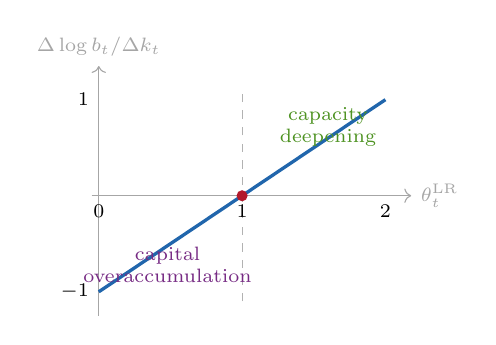
\begin{tikzpicture}[x=1.82cm,y=1.22cm,font=\scriptsize]
        \draw[->,gray!70] (-0.05,0) -- (2.18,0) node[right] {$\theta_t^{\LR}$};
        \draw[->,gray!70] (0,-1.25) -- (0,1.35) node[above] {$\Delta\log b_t/\Delta k_t$};
        \draw[very thick,pathblue] (0,-1) -- (2,1);
        \draw[dashed,gray!60] (1,-1.1) -- (1,1.1);
        \fill[pathred] (1,0) circle (2pt);
        \node[below] at (0,0) {$0$};
        \node[below] at (1,0) {$1$};
        \node[below] at (2,0) {$2$};
        \node[left] at (0,-1) {$-1$};
        \node[left] at (0,1) {$1$};
        \node[align=center,pathpurple] at (0.48,-0.72) {capital\\overaccumulation};
        \node[align=center,pathgreen] at (1.60,0.72) {capacity\\deepening};
      \end{tikzpicture}
      \begin{alertblock}{Admissibility}
        Contraction years are classified separately; they do not mechanically reverse the threshold interpretation.
      \end{alertblock}
    \end{column}
  \end{columns}
  \sourcefooter{Chapter identification architecture, Harrodian benchmark at source line \LineHarrodianBenchmark}
\end{frame}

% Main 9
\begin{frame}{$\theta_t$ classifies accumulation; $\mu_t$ classifies realized use}
  \vspace{-0.25em}
  \begin{block}{Utilization dynamics after capacity reconstruction}
    \centering
    \Large $\Delta\log\mu_t=\Delta y_t-\theta_t^{\LR}\Delta k_t$
  \end{block}
  \scriptsize
  \renewcommand{\arraystretch}{1.45}
  \begin{tabular}{@{}L{0.18\textwidth}L{0.37\textwidth}L{0.37\textwidth}@{}}
    \toprule
    & \centering\arraybackslash $\mu_t<1$: unused capacity
    & \centering\arraybackslash $\mu_t>1$: capacity strain \\
    \midrule
    $\theta_t^{\LR}<1$\\capital overaccumulation
      & \textbf{Overaccumulation with slack.} Weak capacity conversion coexists with a demand shortfall large enough to leave installed capacity unused.
      & \textbf{Overaccumulation with strain.} Capital accumulates faster than capacity while realized demand presses against the available envelope. \\
    $\theta_t^{\LR}>1$\\capacity deepening
      & \textbf{Realized excess capacity.} Capacity grows more than proportionally and effective demand fails to absorb it.
      & \textbf{Expansion absorbed by demand.} High capacity conversion is matched by realized output, preventing unused capacity. \\
    \bottomrule
  \end{tabular}
  \vspace{0.35em}
  \begin{columns}[T,onlytextwidth]
    \begin{column}{0.49\textwidth}
      \centering $g_{\mu,t}<0$: movement toward greater slack
    \end{column}
    \begin{column}{0.49\textwidth}
      \centering $g_{\mu,t}>0$: movement toward greater strain
    \end{column}
  \end{columns}
  \begin{alertblock}{The thresholds answer different questions}
    $\theta_t^{\LR}$ identifies how accumulation builds capacity. The anchored level and movement of $\mu_t$ identify whether that capacity is used.
  \end{alertblock}
  \sourcefooter{Distribution-conditioned identification sequence and explicit capacity anchoring}
\end{frame}

% Main 10
\begin{frame}{A regime claim requires uncertainty to clear unity}
  \small
  \renewcommand{\arraystretch}{1.5}
  \begin{tabular}{@{}L{0.25\textwidth}L{0.29\textwidth}L{0.38\textwidth}@{}}
    \toprule
    \textbf{Simultaneous band} & \textbf{Decision rule} & \textbf{Structural verdict} \\
    \midrule
    entirely below unity & $U_t^{\theta}<1$ & below-one capital-overaccumulation regime \\
    crosses unity & $L_t^{\theta}\leq1\leq U_t^{\theta}$ & indeterminate; the data do not identify a side of the benchmark \\
    entirely above unity & $L_t^{\theta}>1$ & above-one capacity-deepening regime \\
    \bottomrule
  \end{tabular}

  \vspace{0.8em}
  \begin{columns}[T,onlytextwidth]
    \begin{column}{0.48\textwidth}
      \begin{block}{Structural classification also fails when}
        \begin{itemize}\small
          \item the accumulated-path rank condition fails;
          \item the long-run residual is nonstationary;
          \item $\theta_t^{\LR}\leq0$;
          \item cumulative capital growth is nonpositive.
        \end{itemize}
      \end{block}
    \end{column}
    \begin{column}{0.48\textwidth}
      \begin{alertblock}{Final analytical verdict}
        $\theta_t^{\LR}>1$ establishes a tendency for capacity to outrun capital. Actual unused capacity requires $\mu_t<1$ or a sustained $g_{\mu,t}<0$.
      \end{alertblock}
    \end{column}
  \end{columns}
  \sourcefooter{Theta-recovery admissibility rule and generated-state inference contract}
\end{frame}

\appendix

% Appendix 1
\begin{frame}{A1. Identification fails when any gate fails}
  \scriptsize
  \renewcommand{\arraystretch}{1.35}
  \begin{tabular}{@{}L{0.18\textwidth}L{0.39\textwidth}L{0.35\textwidth}@{}}
    \toprule
    \textbf{Gate} & \textbf{Pass condition} & \textbf{Failure classification} \\
    \midrule
    state order & $k_t$ and $Q_t^{tech}$ are admissible long-run states & mixed-order or polynomial-risk specification \\
    rank & $\operatorname{rank}[k_t,Q_t^{tech}]=2$ & technique path is not separately identified from scale \\
    residual & $\widehat\varepsilon_t\sim I(0)$ & no stable long-run capacity relation \\
    timing & $q_{t-1}^*$ weights $\Delta k_t$ & contemporaneous reverse-causality risk \\
    anchoring & one explicit benchmark fixes the level of $y_t^p$ & $\mu_t$ remains underidentified \\
    economic range & simultaneous band remains above zero & economically inadmissible capacity payoff \\
    accumulation & $\sum_{t\in w}\Delta k_t>0$ & no threshold interpretation for that window \\
    \bottomrule
  \end{tabular}
  \vspace{0.7em}
  \begin{block}{Rank has an economic meaning}
    Technique must vary when accumulation occurs. If $\widetilde q_{t-1}^*\Delta k_t$ is only a constant multiple of $\Delta k_t$, the data identify scale but not a separate technique-conditioned elasticity.
  \end{block}
  \sourcefooter{Capacity-utilization identification rule and theta-recovery admissibility ledger}
\end{frame}

% Appendix 2
\begin{frame}{A2. Composition payoffs and annual ratios cannot classify the regime}
  \begin{block}{Two-capital differential}
    \centering
    \Large
    $\displaystyle
    d y_t^p
    =\theta_t^{scale}\,d k_t^{NR}
    +\theta_t^{\tau}\,d\tau_t,
    \qquad
    \tau_t=k_t^{ME}-k_t^{NR}$
  \end{block}
  \footnotesize
  \renewcommand{\arraystretch}{1.20}
  \begin{tabular}{@{}L{0.25\textwidth}L{0.35\textwidth}L{0.32\textwidth}@{}}
    \toprule
    \textbf{Object} & \textbf{Counterfactual answered} & \textbf{Regime role} \\
    \midrule
    $\theta_t^{\LR}$ & How much does capacity change when productive capital expands along the long-run accumulation path? & structural coefficient tested against one \\
    $\theta_t^{\tau}$ & What is the capacity payoff of changing ME/NR composition at a given scale? & composition mechanism, not aggregate regime threshold \\
    $g_t^p/g_t^{cap}$ & What capacity payoff occurred along this particular annual direction? & realized-direction diagnostic, not an equilibrium coefficient \\
    \bottomrule
  \end{tabular}
  \vspace{0.4em}
  \textbf{Balanced-accumulation verdict:} Holding composition fixed gives $d\tau_t=0$. The scale derivative remains; the composition payoff and the annual denominator do not enter the unity test.
  \sourcefooter{Theta-recovery component-capital ledger and the long-run object distinction}
\end{frame}

% Appendix 3
\begin{frame}{A3. Generated-state uncertainty must be propagated end to end}
  \centering
  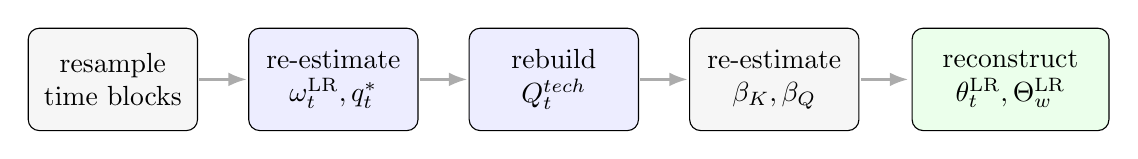
\begin{tikzpicture}[>=Latex, every node/.style={align=center}]
    \draw[->,thick,gray!65] (2.15,0) -- (2.75,0);
    \draw[->,thick,gray!65] (4.95,0) -- (5.55,0);
    \draw[->,thick,gray!65] (7.75,0) -- (8.35,0);
    \draw[->,thick,gray!65] (10.55,0) -- (11.15,0);
    \node[draw,rounded corners,fill=gray!7,minimum width=2.15cm,minimum height=1.30cm] at (1.05,0)
      {resample\\time blocks};
    \node[draw,rounded corners,fill=blue!7,minimum width=2.15cm,minimum height=1.30cm] at (3.85,0)
      {re-estimate\\$\omega_t^{\LR},q_t^*$};
    \node[draw,rounded corners,fill=blue!7,minimum width=2.15cm,minimum height=1.30cm] at (6.65,0)
      {rebuild\\$Q_t^{tech}$};
    \node[draw,rounded corners,fill=gray!7,minimum width=2.15cm,minimum height=1.30cm] at (9.45,0)
      {re-estimate\\$\beta_K,\beta_Q$};
    \node[draw,rounded corners,fill=green!8,minimum width=2.50cm,minimum height=1.30cm] at (12.45,0)
      {reconstruct\\$\theta_t^{\LR},\Theta_w^{\LR}$};
  \end{tikzpicture}

  \vspace{0.7em}
  \begin{block}{Window-level long-run elasticity}
    \centering
    \Large
    $\displaystyle
    \Theta_w^{\LR}
    =
    \frac{\sum_{t\in w}\theta_t^{\LR}\Delta k_t}
         {\sum_{t\in w}\Delta k_t},
    \qquad
    \sum_{t\in w}\Delta k_t>0$
  \end{block}
  \begin{columns}[T,onlytextwidth]
    \begin{column}{0.47\textwidth}
      \begin{block}{Bootstrap protocol}
        \BootstrapReplications\ moving-block draws with block length \BootstrapBlockLength\ years. Every draw re-estimates the complete generated-regressor chain.
      \end{block}
    \end{column}
    \begin{column}{0.50\textwidth}
      \begin{block}{Inference output}
        \SimultaneousBandLevel\% simultaneous bands for $\theta_t^{\LR}$ and bootstrap intervals for $\Theta_w^{\LR}$. Pointwise intervals alone do not identify sustained regimes.
      \end{block}
    \end{column}
  \end{columns}
  \sourcefooter{Generated-state inference contract; \AnalyticalClaimCount\ source claims and \AnalyticalIdentityCount\ identities validated}
\end{frame}

\end{document}
